\begin{figure}[p]
	\centering

	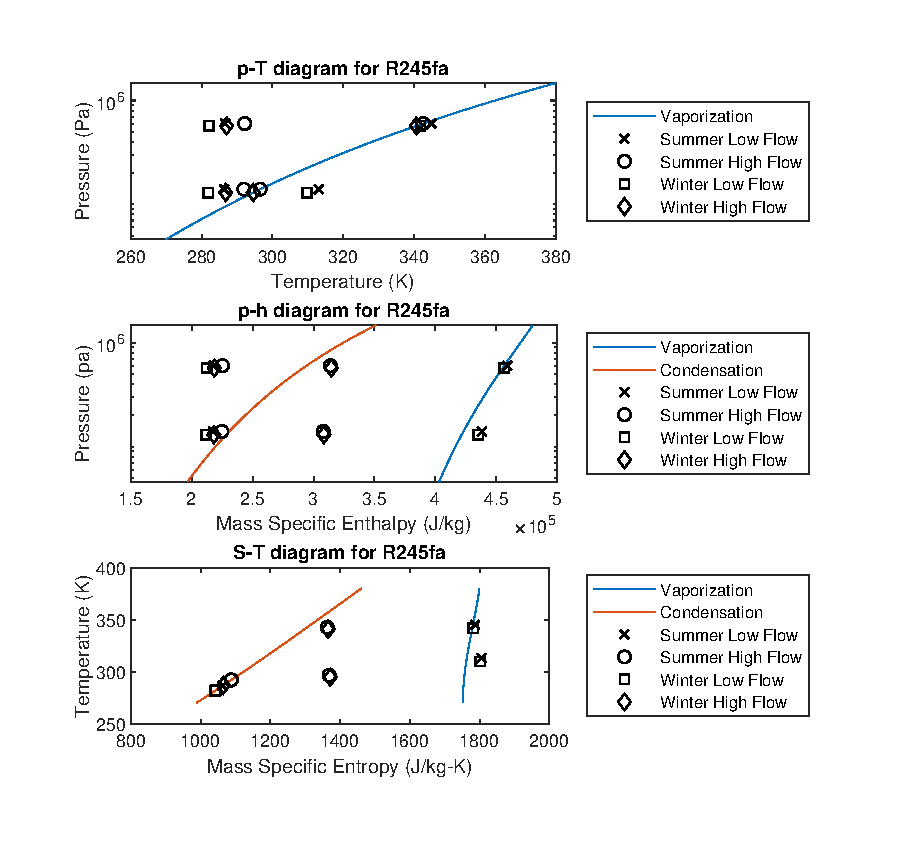
\includegraphics[width=\textwidth]{figures/GreenfieldThermoPlots}
	%\includegraphics{figures/VerificationPH01}
	\caption{Thermodynamic plots from the greenfield ORC prime power system which includes pressure against temperature (top), pressure against mass specific enthalpy (middle), and temperature against mass specific entropy (bottom). All points assume a source temperatures of \SI{364.5}{\kelvin} (\SI{91}{\degreeCelsius}), as well as source and sink flow rates of \SI{940}{\liter\per\minute}. Sink temperatures are assumed to be \SI{276.6}{\kelvin} (\SI{3.5}{\degreeCelsius}) in Winter and \SI{281.6}{\kelvin} (\SI{8.5}{\degreeCelsius}) in Summer. High flow rate points have a working fluid mass flow rate of approximately \SI{8.4}{\kilogram\per\second}}
\label{fig:gf_themoplots}
\end{figure}